\chapter {Implementation of Modbus Protocol}
\thispagestyle{empty}
\label{modbus}

\newcommand{\LocMODfig}{\Origin/user-code/modbus/figures}
\newcommand{\LocMODscicode}{\Origin/user-code/modbus/scilab}
\newcommand{\LocMODscibrief}[1]{{\tt \seqsplit{%
Origin/user-code/modbus/scilab}}, see \fnrefp{fn:file-loc}}
\newcommand{\LocMODardcode}{\Origin/user-code/modbus/arduino}
\newcommand{\LocMODardbrief}[1]{{\tt \seqsplit{%
Origin/user-code/modbus/arduino}}, see \fnrefp{fn:file-loc}}

%%%%%%%%%%%%python starts
\newcommand{\LocMODpycode}{\Origin/user-code/modbus/python}
\newcommand{\LocMODpybrief}[1]{{\tt \seqsplit{%
Origin/user-code/modbus/python}}, see \fnrefp{fn:file-loc}}
%%%%%%%%%%%%python ends

%%%%julia starts

\newcommand{\LocMODjuliacode}{\Origin/user-code/modbus/julia}
\newcommand{\LocMODjuliabrief}[1]{{\tt \seqsplit{%
Origin/user-code/modbus/julia}}, see \fnrefp{fn:file-loc}}

%%%%julia ends


%%%%OpenModelica starts

\newcommand{\LocMODOpenModelicacode}{\Origin/user-code/modbus/OpenModelica}
\newcommand{\LocMODOpenModelicabrief}[1]{{\tt \seqsplit{%
Origin/user-code/modbus/OpenModelica}}, see \fnrefp{fn:file-loc}}

%%%%OpenModelica ends

In this chapter we will learn one of the advanced applications that
can be built using Scilab-Arduino toolbox. Beginners might want to
skip this chapter in the first reading. This experiment enables
interfacing Modbus based devices with Scilab-Arduino toolbox. This
functionality has a wide number of applications in the industrial
sector.

\section{Preliminaries}
Modbus is an open serial communication protocol developed and
published by Modicon in 1979. Because of ease of deployment and
maintenance, it finds wide applications in industries. The Modbus
protocol provides a means to transmit information over serial lines
between several electronic devices in order to control and monitor
them. The controlling device requests for reading or writing
information and is known as the Modbus Master/Client. On the other
hand, the device or devices supplying the information are called
Modbus Slaves/Server. All the slaves/servers have a unique id and
address. Typically, there is one Master and maximum 247 Slaves.

During the communications on a Modbus network, the protocol determines
how the controller gets to know its device address, recognizes the
message provided and decides the action to be taken and accordingly
extracts data and information contained in the message. The data is
sent as a series of zeros and ones, i.e. bits wherein zeros are sent
as positive voltages and ones as negative.

Different versions of Modbus protocol exist on serial lines, namely
Modbus RTU, ASCII and TCP. The Energy Meter used in this experiment
supports Modbus RTU protocol. In Modbus RTU, the data is coded in
binary and requires only one communication byte. This is ideal for use
over RS232 or RS485 networks at baud rates between 1200 and 115K.

\begin{figure}
\centering
%\subfloat[Block diagram representation of the Protocol]{
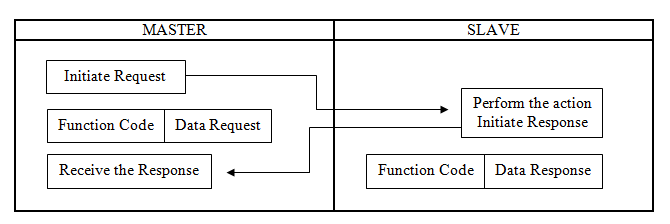
\includegraphics[width=\hgfig]{\LocMODfig/fig1.png}
\label{fig:mod-block}
\caption{Block diagram representation of the Protocol}
\end{figure}


\begin{figure}
\centering
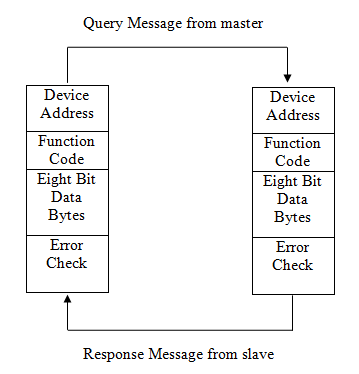
\includegraphics[width=\smfig]{\LocMODfig/fig2.png}
\caption{Master-Slave Query-Response Cycle}
\label{fig:mod-master-slave}
\end{figure}

The RS485 is one of the most widely used bus standards for industrial
applications. It uses differential communication lines to communicate
over long distances and requires a dedicated pair of signal lines, say
A and B, to exchange information. Here, the voltage on one line equals
to the inverse of the voltage on the other line. In other words, the
output is,
1, if A-B\textgreater200mV, and 0, if B-A\textgreater200mV.

%\begin{center}
%\framebox(175,30){%
 %   \parbox{170\unitlength}{R0 outputs 1, if A-B\textgreater200mV\\ R0 outputs 0, if B-A\textgreater200mV}%
%}
%\end{center}

%\begin{align*}
%R0 outputs 1, if A-B\textgreater200mV\\
%R0 outputs 0, if B-A\textgreater200mV
%\end{align*}


\begin{figure}
\centering
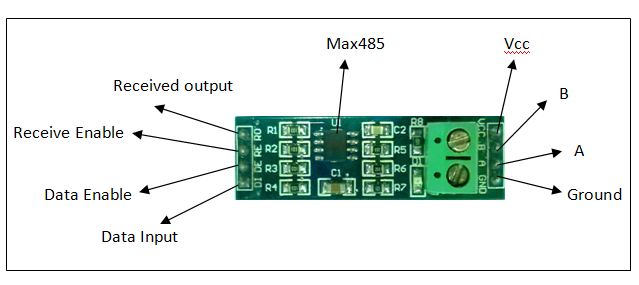
\includegraphics[width=\hgfig]{\LocMODfig/fig3.png}
\caption{Pins in RS485 module}
\label{fig:rs-485}
\end{figure}

Energy Meter is a device that measures amount of electricity consumed
by the load. We are using Energy Meter EM6400, which is a
multifunction digital power meter by Schneider Electric India. It
reads various parameters such as phase voltage, current, active power,
reactive power, power factor etc. Before using the meter, one has to
program system configuration, PT, CT ratios, communication parameters
through front panel keys. EM6400 supports Modbus for communication.

Multiple operations can be performed with devices supporting
Modbus. Every operation has its own fixed function code (coil
status-01, input status-02, holding registers-03, input registers-04,
etc.), which is independent of devices. All the parameter values are
stored in the holding registers. Different holding registers hold
values of different parameters. Individual parameter addresses can be
found in user manual for EM6400.  
For example,
\begin{center}
\begin{tabular}{ll}
Current (phase 1): & 3929 \\
Voltage (phase 1): & 3927 \\
Active power (phase 1): & 3919
\end{tabular}
\end{center}

The size of each Modbus register is 16 bits and all EM6400 readings
are 32 bits. So, each reading occupies two consecutive Modbus
registers. Values in every register are in little endian format (1st
register contains LSB and next register contains MSB). In our case,
Energy Meter is a slave and slave addresses can be set between 1 and
247.

A request to read holding registers has to be sent in a specified
format. An example of a request packet is as follows.  Suppose that
the request is 01 03 0F56 0002 270F.  Its meaning is explained in
\tabref{tab:request-packet}.
\begin{table}
\centering
\caption{Interpretation of a request packet}
\label{tab:request-packet}
\begin{tabular}{lp{10cm}}
01 &  Slave address \\
03 & Function code to read holding registers \\
0F56 & Data Address of the first requested register (address for
voltage phase1 to neutral) and 
(0F56 hex = 3927, +40001 offset = 43928) \\
0002 & Total number of registers requested for read \\
270F & CRC (Cyclic Redundancy Check) for error checking (LSB first) \\
\end{tabular}
\end{table}
The response packet corresponding the above request packet
is given as 01 03 04 2921 4373 D2B0.  Its meaning is explained in
\tabref{tab:response-packet}.
\begin{table}
\centering
\caption{Interpretation of a response packet}
\label{tab:response-packet}.
\begin{tabular}{ll}
01 & Slave address \\
03 & Function code to read holding registers \\
04 & Total number of bytes read   \\
2921 & Data in 1st requested register \\
4373 & Data in 2st requested register \\
D2B0 & CRC for error checking (LSB first)
\end{tabular}
\end{table}

Values in required registers are 43732921 in hex (since obtained
values are being read in little endian format) which is 243.16 when
converted to floating point using IEEE 754 norms. Obtained value is a
voltage (phase1 to neutral) which is 243.16 Volts.  

Most of the numeric values to be stored in the computer are more than
one byte long. Thus, there arises a question of how to store the
multibyte values on the computer machines where each byte has its own
address i.e. which byte gets stored at the ''first'' (lower) memory
location and which bytes follow in higher memory locations. For
example, if a two byte integer 0x5E5F is stored on disk by one machine
with the 0x5E (high byte or MSB) stored at the lower memory address
and the 0x5F (low byte or LSB) stored at a higher memory address, but
a different machine reads that integer by picking 0x5F for the high
byte and the 0x5E for the low byte, giving 0x5F5E, thus resulting into
an disagreement on the value of the integer between the two
machines. However, there is no so called ''right'' ordering to store
the bytes in the case of multibyte quantities. Hardware is built to
store the bytes in a particular fashion and as long as compatible
hardware reads the bytes in the same fashion, things are
fine. Following are the two major types of byte ordering: 

\begin{description}
\item [Little Endian:]
If the hardware is designed so that the lowest or the least
significant byte (LSB) of a multibyte integer is stored ''first'', at
the lowest memory address, then the hardware is said to be Little
Endian. In this format, the ''little'' end of the integer gets stored
first and the next bytes get stored in higher (increasing) memory
locations.  
\item [Big Endian:]
Here, the hardware is designed so that the highest or the most
significant byte (MSB) of a multibyte integer is stored ''first'', at
the lowest memory address. Thus, the ''big'' end of the integer gets
stored first and accordingly the next bytes get stored in higher
(increasing) memory locations.  
\end{description}
For example, let us take a four byte integer 0x436B84A3. Quite
obvious, the ''little'' end byte, LSB is 0x84A3, and the ''big'' end
byte, MSB is 0x436B; taking into consideration that the Read Holding
Registers are 16 bits each. Thus the aforesaid memory storage patterns
for the integer would be \tabref{tab:ieee-decimal}.

\begin{table}
\centering
\caption{Hexadecimal to Decimal}
\label{tab:ieee-decimal}
\begin{tabular}{ |p{3cm}|p{3cm}|p{3cm}|p{3cm}|}

\hline
\multicolumn{4}{|c|}{Four Bytes Integer Reading from Meter} \\
\hline

            Memory Address & Memory Address & Little Endian & Big Endian \\ \hline
            3900 & 8A43 & MSB & LSB \\
            3901 & 436B & LSB & MSB \\ \hline
          \end{tabular}
\end{table}


In order to represent the Hexadecimal values of the Read Holding
Registers into user friendly decimal (floating point) values, we
follow IEEE 754 Standard. Most common standards for representing
floating point numbers are:
\begin{enumerate}
\item Single Precision: Used for 32 bits. Out of those 32 bits, one
  bit represents the sign bit, 8 bits for exponent and the remaining
  23 bits for mantissa, as depicted in \tabref{tab:single-precision}.

\begin{table}
\centering
\caption{Single and Double Precision Representation}
\label{tab:single-precision}
\begin{tabular}{|l|l|l|l|}
\hline
Single & Sign (1 bit) & Exponent (8 bit) & Mantissa (23 bit) \\ \hline 
Double & Sign (1 bit) & Exponent (11 bit) & Mantissa (52 bit) \\ \hline
\end{tabular}
\end{table}
\item Double Precision: Used for 64 bits. Out of those 32 bits, one bit represents the sign bit, 8 bits for exponent and the remaining 23 bits for mantissa, as depicted in \tabref{tab:single-precision}.
\end{enumerate}
Finally, the decimal value is given by, 
Decimal Value = $( - 1) * \text{sign} * 2^{exponent}* \text{Mantissa}$.
Hence, for 32 bit values, the sign is stored in bit 32. The exponent
can be calculated from bits 24-31 by subtracting 127. The mantissa is
stored in bits 1-23. An invisible leading bit (i.e. it is not actually
stored) with value 1.0 is placed in front, then bit 23 has a value of
1/2, bit 22 has value 1/4 etc. As a result, the mantissa has a value
between 1.0 and 2. At last, the decimal value is calculated using the
above mentioned equation. Though there are several online converters
available as IEEE 754 Converter, a function has been formulated in
Scilab for this conversion here.  


\section{Objective}
The objective of this experiment is to make the user acquainted with
the use of Modbus protocol through Arduino Uno. It gives an insight on
how to acquire readings from the Energy Meter and interpret them
accordingly. As mentioned earlier, an Energy Meter is a device that
gives us different electrical parameters including voltage, current,
and power, consumed by a device. Here, we aim to obtain these values
using Scilab and Arduino Uno. For data transmission, we have used
RS485 Module.

Scilab is used for giving the required parameters to Arduino Uno. For
example, the user will tell the required Slave Address to be accessed
and the number of registers to be read from or written to. Here,
Arduino Uno acts as a master and Energy Meter as a slave. Therefore,
referring to a particular slave address will refer to the registers
that hold the desired electrical parameters (Current, Voltage, Power
etc.), which we want from the Energy Meter (Slave).

This Arduino Uno is then connected to the Energy Meter via a MAX485
chip which facilitates long distance communication. The information
packet is sent to the Arduino Uno, which in turn sends it to the
Energy Meter. The Energy Meter then accesses the values in the
required addresses in its memory and transfers them back. This again,
is in the form of another packet. Data which is in Little Endian hex
format is obtained from this and is converted to floating point number
using IEEE 754.

\begin{figure}
\centering
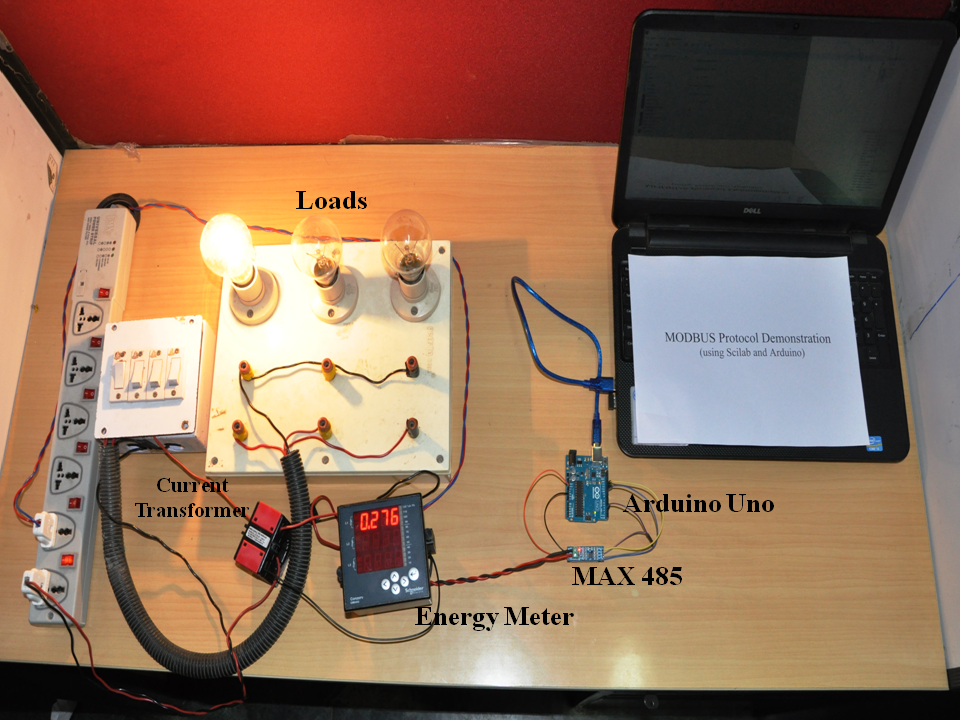
\includegraphics[width=\lgfig]{\LocMODfig/Full-Set-Up.png}
\caption{MODBUS Set Up for Energy Meter}
\label{fig:full-set-up}
\end{figure}

\section{Energy Meter set up for Modbus protocol with Arduino Uno}
\begin{enumerate}
\item As we know, Arduino Uno has one serial port. It communicates on
  the digital pins 0 and 1 as well as on the computer via USB. Since
  we want serial communication which shouldn't be disturbed by the USB
  port and the Serial Monitor, we use the Software Serial
  library. Using this library we can assign any digital pins as RX and
  TX and use for serial communication. Pin 10 (used as RX) and Pin
  11(used as TX) is connected to RO (Receive Out) and DI (Data In)
  pins of MAX485 module respectively.
\item DE (Data Enable) and RE (Receive Enable) pins of RS 485 are
  shorted and connected to digital pin 3 of Arduino Uno. This serves
  as Control Pin which will control when to receive and transmit
  serially.
\item Vcc and GND of the MAX485 module are connected to Vcc and GND of
  Arduino.
\item A and B pins of MAX485 are connected to A (Pin 7) and B (Pin 14)
  pins of the Energy Meter (meant for RS485 communication).
\item A $120k\Omega$ termination resistance is connected in between
  pins A and B to avoid reflection losses in transmission line.
\end{enumerate}

\begin{figure}
\centering
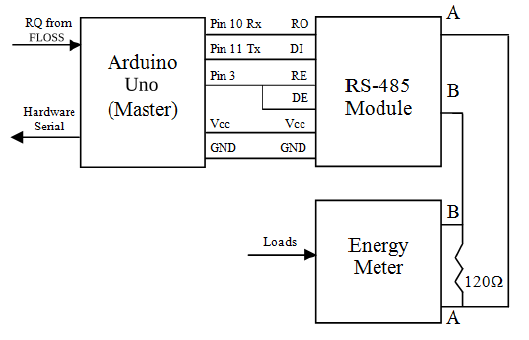
\includegraphics[width=\lgfig]{\LocMODfig/block-diagram.PNG}
\caption{Block Diagram for Energy Meter Setup}
\label{fig:block-diagram}
\end{figure}

\section{Software}

Software for the demonstration comprises two parts:

\begin{enumerate}
\item Arduino Uno firmware code: This code is written to communicate
  with Scilab (using serial interface), and with MAX485 chip (using
  Software Serial interface). Control logic to enable receive and
  transmit modes of MAX485 chip is also present in Arduino Uno
  firmware code.The overall implementation is being described in
  \figref {fig:modbus-firmware}.

\begin{figure}
\centering
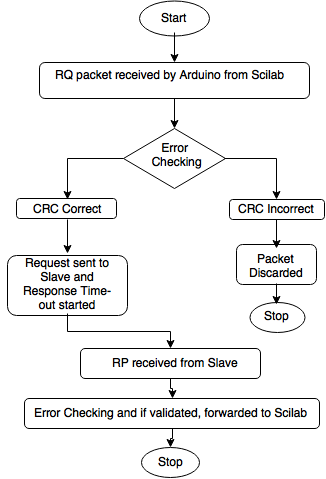
\includegraphics[width=\lgfig]{\LocMODfig/arduino_code_flowchart.png}
\caption{Flowchart of Arduino firmware}
\label{fig:modbus-firmware}
\end{figure}

\item Scilab code: This code requests Energy Meter readings by sending
  request packet to Arduino Uno from Scilab. Then it waits till
  requested packet is available from Arduino Uno. After receiving the
  packet, it extracts data from the packet and converts it into IEEE
  754 floating point format. The overall implementation is being
  described below:

\begin {enumerate}
\item Frame request packet to be sent to slave in ASCII coded decimal
  format
\item Send the packet serially to Arduino Uno board (Arduino Uno sends
  this packet to Energy Meter via RS 485 module)
\item Read the response packet available on Arduino Uno board (sent by
  Energy meter to Arduino via RS 485)
\item Extract holding register contents from received packet
\item Convert 32 bit register contents which are in little endian
  format to floating point number using ieeesingle2num function
\item Display the value of electrical parameter read(i.e. voltage,
  current or power)
\end{enumerate}

\begin{figure}
\centering
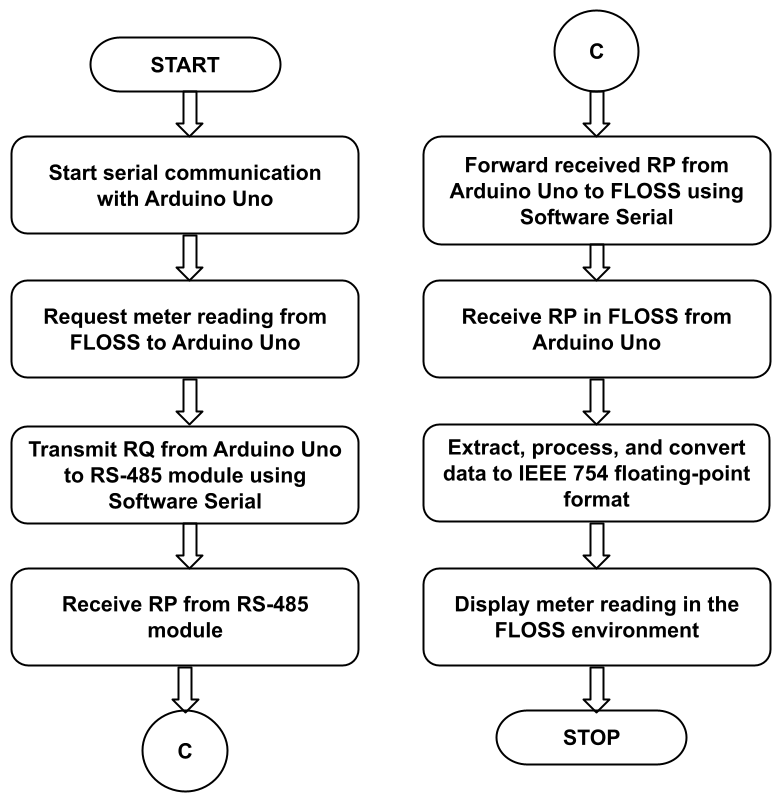
\includegraphics[width=\hgfig]{\LocMODfig/flowchart.png}
\caption{Flow Chart of the Modbus Energy Meter Implementation}
\label{fig:flow-chart}
\end{figure}

\end{enumerate}

\section{Output}

\begin{enumerate}
\item Single phase current output: \figref{fig:current-console} and
  \figref{fig:current-meter} show Scilab code output of current in
  Amperes and corresponding snapshot of Energy Meter display with a
  single load rated 60W-230V.

\begin{figure}
\centering
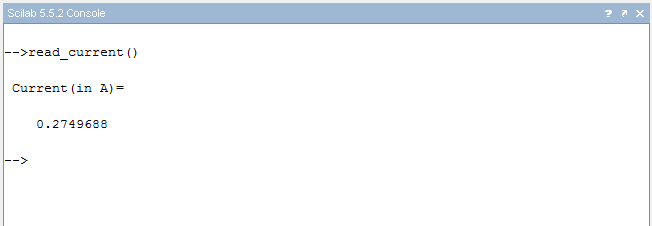
\includegraphics[width=\linewidth]{\LocMODfig/current-output.png}
\caption{Single Phase Current Output on Scilab Console}
\label{fig:current-console}
\end{figure}

\begin{figure}
\centering
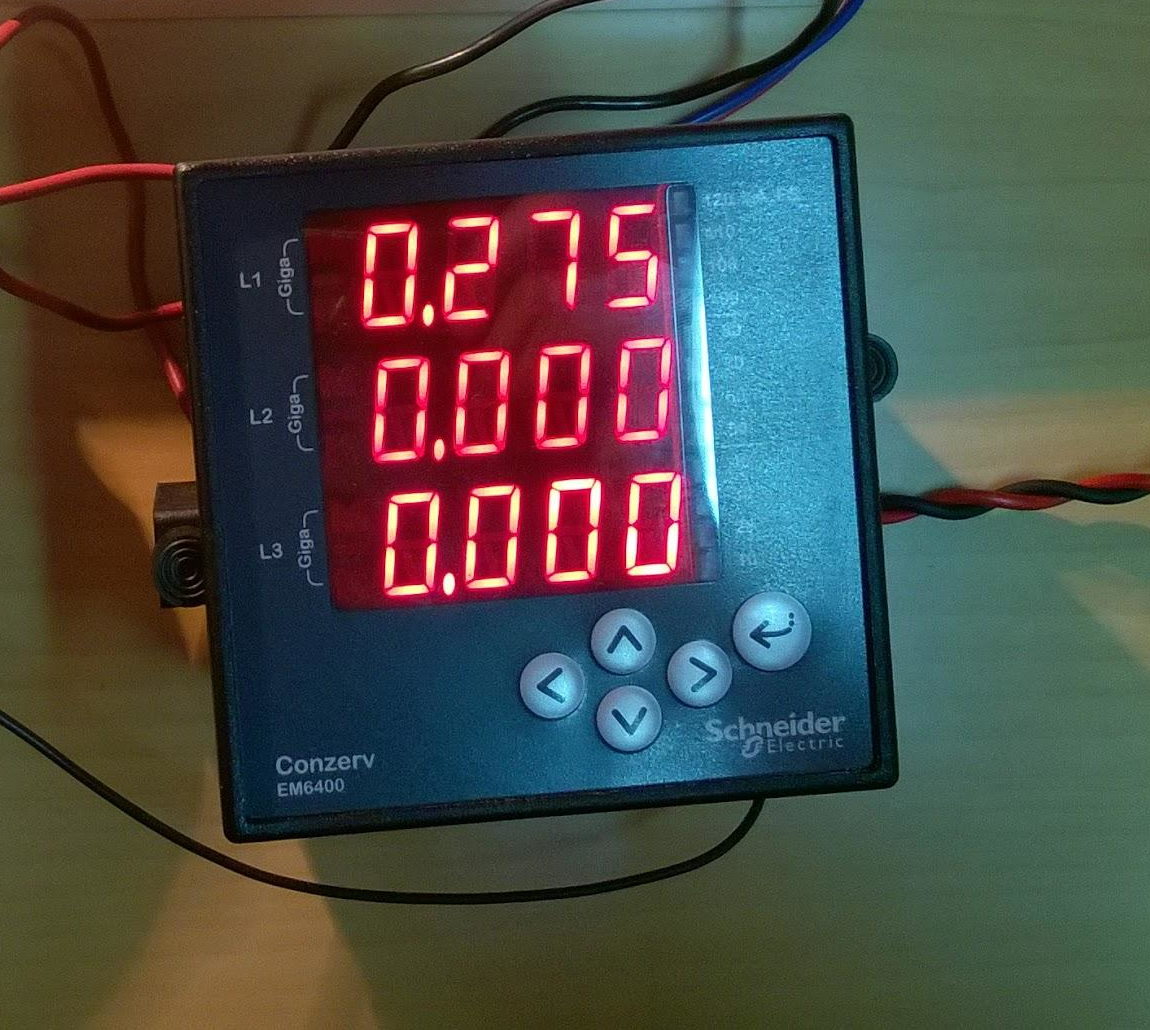
\includegraphics[width=\lgfig]{\LocMODfig/current-output-setup.jpg}
\caption{Single Phase Current Output on Energy Meter}
\label{fig:current-meter}
\end{figure}

\item Single phase voltage output: \figref{fig:voltage-console} and
  \figref{fig:voltage-meter} show Scilab code output of voltage in
  Volts and corresponding snapshot of Energy Meter display with a
  single load rated 60W-230V.

\begin{figure}
\centering
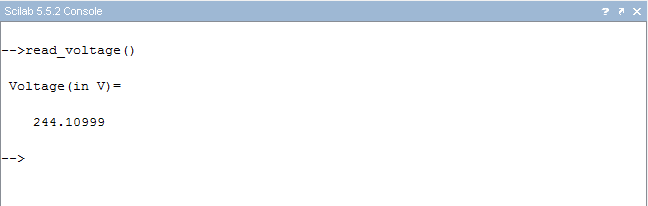
\includegraphics[width=\linewidth]{\LocMODfig/voltage-output.png}
\caption{Single Phase Voltage Output on Scilab Console}
\label{fig:voltage-console}
\end{figure}

\begin{figure}
\centering
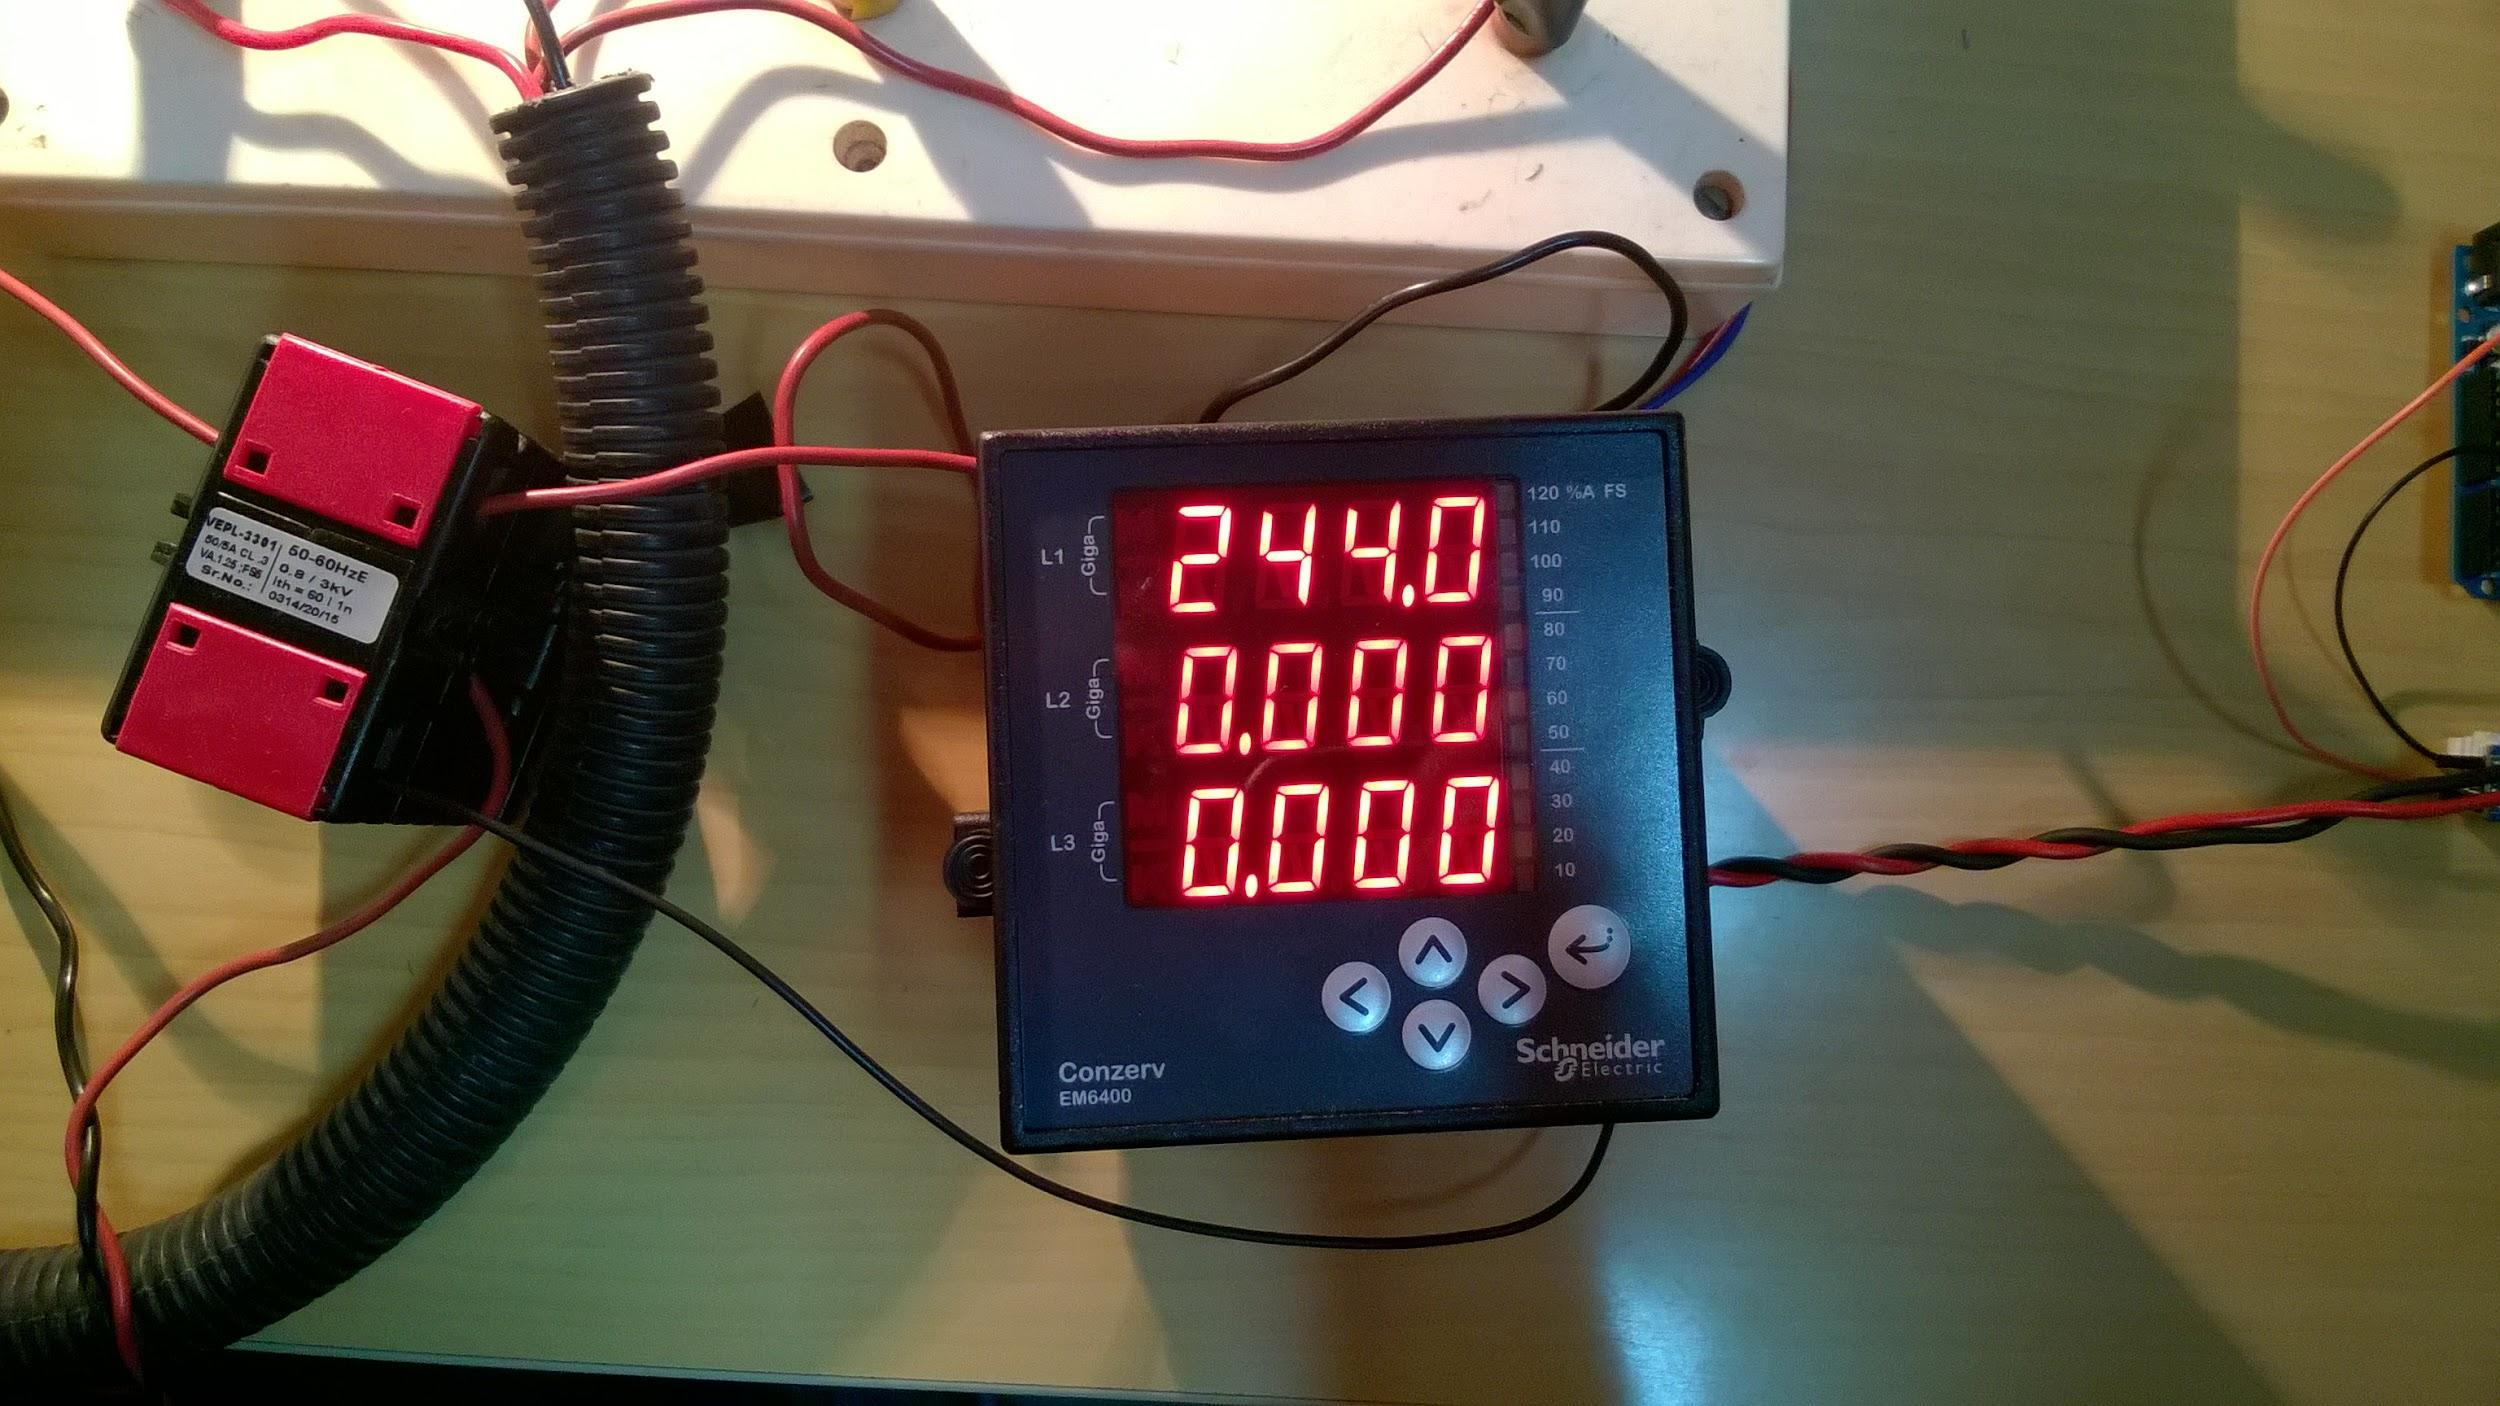
\includegraphics[width=\lgfig]{\LocMODfig/voltage-output-setup.jpg}
\caption{Single Phase Voltage Output on Energy Meter}
\label{fig:voltage-meter}
\end{figure}

\item Single phase active power outputs are shown in
  \figref{fig:power-console} and \figref{fig:power-meter}.

\begin{figure}
\centering
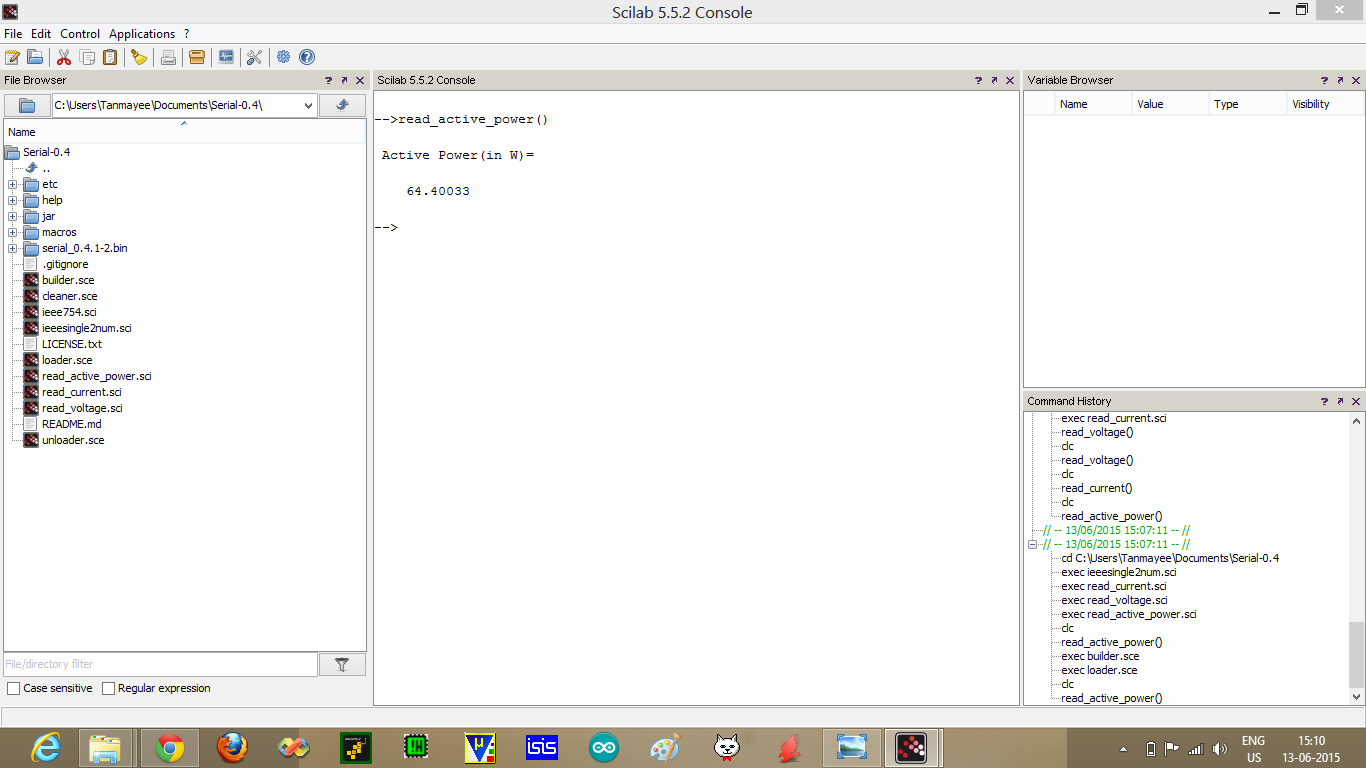
\includegraphics[width=\linewidth]{\LocMODfig/active-power-output.png}
\caption{Single Phase Voltage Output on Scilab Console}
\label{fig:power-console}
\end{figure}

\begin{figure}
\centering
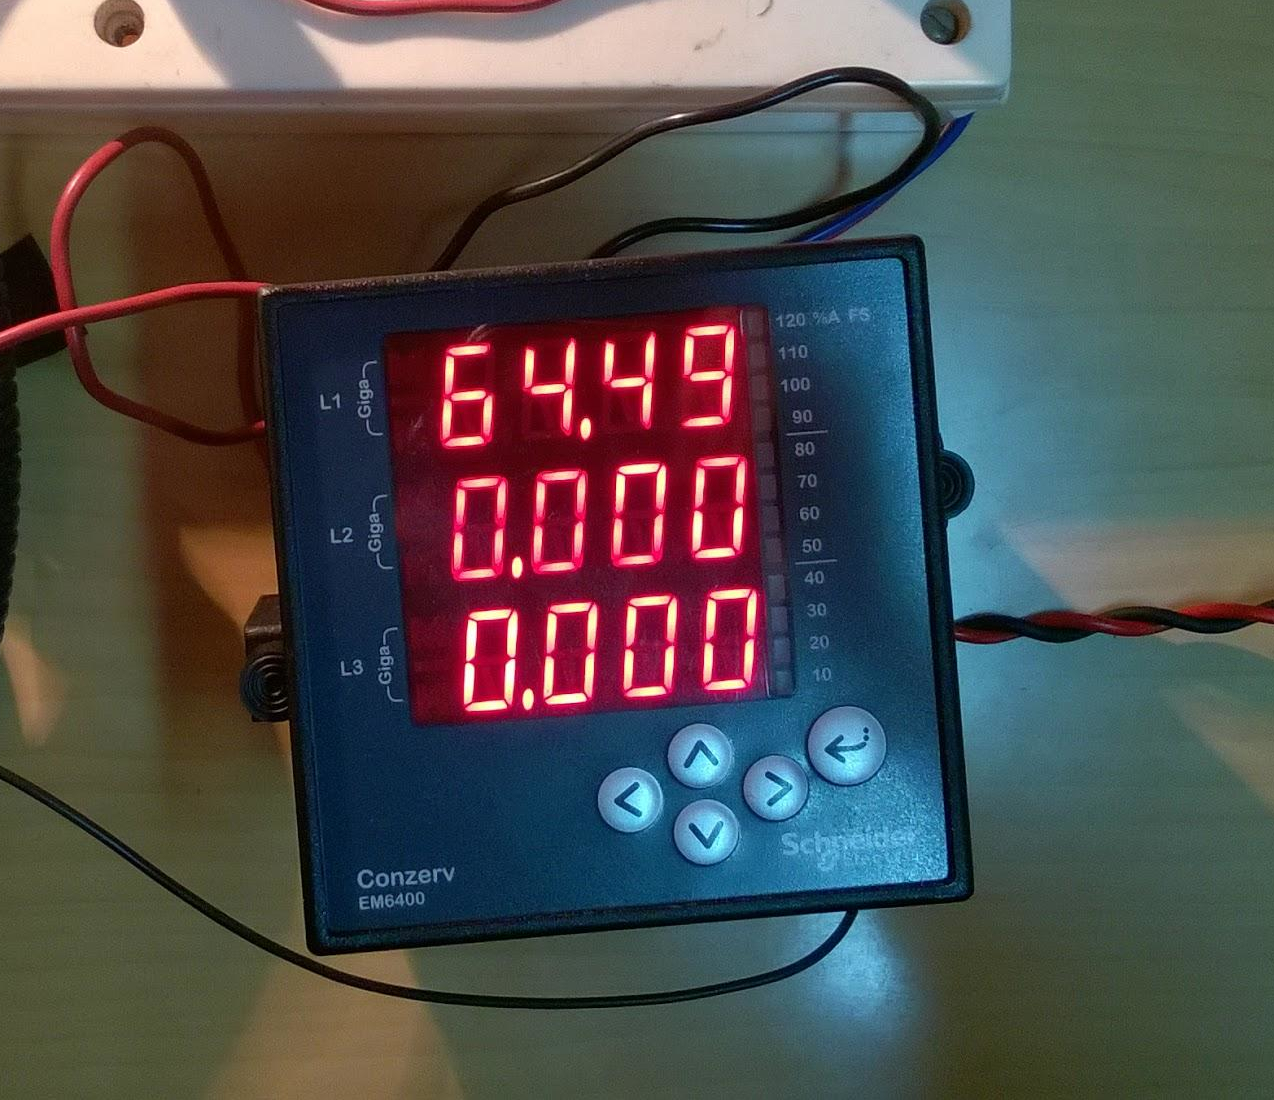
\includegraphics[width=\lgfig]{\LocMODfig/active-power-output-setup.jpg}
\caption{Single Phase Voltage Output on Energy Meter}
\label{fig:power-meter}
\end{figure}

\end{enumerate}


In output, user could see the requested energy parameter on Scilab
console. For demonstration we have taken single phase current, single
phase voltage and single phase active power reading. We can always
verify the Scilab output with the value being displayed on the Energy
Meter display screen.

\section{Reading Parameters from Xcos}
In this section we will carry out the same experiments discussed in
the previous sections but through Xcos. One should go through
\secref{sec:xcos-start} before continuing.

\begin{enumerate}
\item The Xcos diagram for performing the read values for single phase
  current, single phase voltage and single phase power operation is as
  shown in \figref{fig:mod-read}. The location of the xcos file is
  mentioned in the caption of the figure.

\begin{figure}
    \centering
    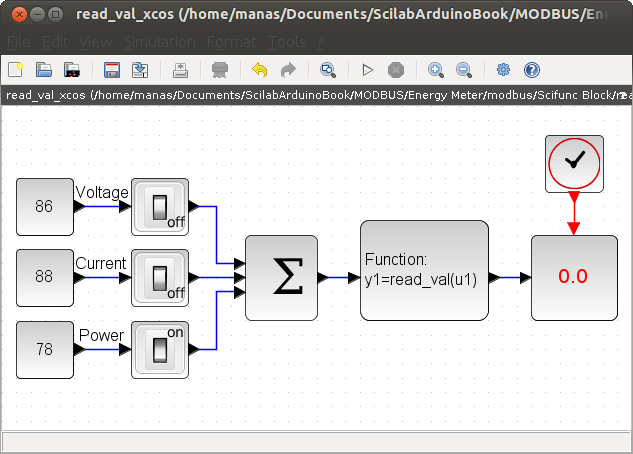
\includegraphics[width=\lgfig]{\LocMODfig/read_value_xcos.png}
    \caption[Xcos diagram to read Energy Meter values]{Xcos diagram to
      read Energy Meter values.  This is what one sees when {\tt
        \LocMODscibrief/read\_value\_xcos.zcos} is invoked.}
    \label{fig:mod-read}
  \end{figure}
The parameters of the blocks can be changed by right clicking on the
block and choosing {\tt Block Parameters}. One can also double click
on the block. The values for each block is tabulated in
\tabref{tab:mod-xcos-read}.  All other parameters are to be left
unchanged.

\begin{table}
    \centering
    \caption{Xcos parameters to read Energy Meter}
    \label{tab:mod-xcos-read}
    \begin{tabular}{llc} \hline
      Name of the block & Parameter name & Value \\ \hline
      CONST\_m & Address byte for voltage & 86  \\
      & Address byte for current & 88 \\ 
      & Address byte for power & 78\\ \hline
      SELF\_SWITCH & Signal Routing & on/off \\ \hline
      BIGSOM\_f & Scalar vector addition/subtraction Summation & [1;1;1] \\ \hline
      scifunc\_block\_m & Block for user\-defined function & read\_value.sci \\ \hline 
      AFFICH\_m & Block inherits(1) or not (0) & 0 \\ \hline
      CLOCK\_c & Period & 0.1 \\
      & Initialisation Time & 0 \\ \hline
    \end{tabular}
  \end{table}
\end{enumerate}

After we send the query using Modbus protocol from Scilab (using
write\_serial command) to the Energy Meter, we will receive a packet
from the Energy Meter which will contain the data requested. This data
is read serially using (read\_serial command) in Scilab and the bytes
so received are stored in the 'buf' variable. On analyzing the bytes
received (by observing the value of ASCII(buf) or myresult) we see
that there might be some spaces(value 32 in myresult) received. So the
required data starts from the fourth byte available excluding
spaces.For example, If there are n spaces received before the packet,
so the required data would be starting at n+4 position(i.e., we have
to analyse the four bytes starting at (n+4)th position). Note that the
packet received may have one or more spaces at the starting or the
ending and that is the reason why we may have to shift our indexing
for analyzing data.

The functionalities performed by scilab code have also been implemetned in 
python and julia and OpenModelica.

\section{Code}
\subsection{Arduino Code}
\label{sec:firmware-modbus}
\addtocontents{ard}{\protect\addvspace{\codclr}}

\begin{ardcode}
\acaption{First 10 lines of the firmware for Modbus Energy Meter
  experiment} 
{First 10 lines of the firmware for Modbus.  Available at
  \LocMODardbrief{send\_packet.ino}.}
\label{ard:firmware-modbus}
\lstinputlisting[firstline=1,lastline=10]
{\LocMODardcode/send_packet.ino}
\end{ardcode}

\subsection{Scilab Code}
\label{sec:modbus-scilab-code}
\addtocontents{cod}{\protect\addvspace{\codclr}}

\begin{scicode}
\ccaption{First 10 lines of the function for scifunc block}
{First 10 lines of the Scifunc block function.  Available at
  \LocMODscibrief{read\_val.sci}.} 
\label{sci:current-modbus}
\lstinputlisting[firstline=1,lastline=10]
{\LocMODscicode/read_val.sce}
\end{scicode}

\begin{scicode}
\ccaption{First 10 lines of the code for Single Phase Current Output}
{First 10 lines of the code for Single Phase Current Output.
  Available at \LocMODscibrief{read\_current.sci}.}
\label{sci:current-modbus}
\lstinputlisting[firstline=1,lastline=10]
{\LocMODscicode/read_current.sci}
\end{scicode}

\begin{scicode}
\ccaption{First 10 lines of the code for Single Phase Voltage Output}
{First 10 lines of the code for Single Phase Voltage Output.
  Available at \LocMODscibrief{read\_voltage.sci}.}
\label{sci:voltage-modbus}
\lstinputlisting[firstline=1,lastline=10]
{\LocMODscicode/read_voltage.sci}
\end{scicode}

\begin{scicode}
\ccaption{First 10 lines of the code for Single Phase Active Power
  Output}{First 10 lines of the code for Single Phase Active Power
  Output.  Available at
  \LocMODscibrief{read\_active\_power.sci}.}
\label{sci:modbus-power}
\lstinputlisting[firstline=1,lastline=10]
{\LocMODscicode/read_active_power.sci}
\end{scicode}

\subsection{Python Code}
\label{sec:modbus-python-code}
\addtocontents{pyd}{\protect\addvspace{\codclr}}

\begin{pycode}
\pcaption{Code for Single Phase Current Output}
{Code for Single Phase Current Output.
  Available at \LocMODpybrief{read\_current.py}.}
\label{py:current-modbus}
\lstinputlisting[firstline=1,lastline=10]
{\LocMODpycode/read_current.py}
\end{pycode}

\begin{pycode}
\pcaption{Code for Single Phase Voltage Output}
{Code for Single Phase Voltage Output.
  Available at \LocMODpybrief{read\_voltage.py}.}
\label{py:voltage-modbus}
\lstinputlisting[firstline=1,lastline=10]
{\LocMODpycode/read_voltage.py}
\end{pycode}

\begin{pycode}
\pcaption{Code for Single Phase Active Power
  Output}{Code for Single Phase Active Power
  Output.  Available at
  \LocMODpybrief{read\_active\_power.py}.}
\label{py:modbus-power}
\lstinputlisting[firstline=1,lastline=10]
{\LocMODpycode/read_active_power.py}
\end{pycode}

\subsection{Julia Code}
\label{sec:modbus-julia-code}
\addtocontents{juliad}{\protect\addvspace{\codclr}}

\begin{juliacode}
\jcaption{Code for Single Phase Current Output}
{Code for Single Phase Current Output.
  Available at \LocMODjuliabrief{readCurrent.jl}.}
\label{julia:current-modbus}
\lstinputlisting[firstline=1,lastline=10]
{\LocMODjuliacode/readCurrent.jl}
\end{juliacode}

\begin{juliacode}
\jcaption{Code for Single Phase Voltage Output}
{Code for Single Phase Voltage Output.
  Available at \LocMODjuliabrief{readVoltage.jl}.}
\label{julia:voltage-modbus}
\lstinputlisting[firstline=1,lastline=10]
{\LocMODjuliacode/readVoltage.jl}
\end{juliacode}

\begin{juliacode}
\jcaption{First 10 lines of the code for Single Phase Active Power
  Output}{First 10 lines of the code for Single Phase Active Power
  Output.  Available at
  \LocMODjuliabrief{readPower.jl}.}
\label{julia:modbus-power}
\lstinputlisting[firstline=1,lastline=10]
{\LocMODjuliacode/readPower.jl}
\end{juliacode}

\subsection{OpenModelica Code}
\label{sec:modbus-OpenModelica-code}
\addtocontents{OpenModelicad}{\protect\addvspace{\codclr}}

\begin{OpenModelicacode}
\mcaption{Code for Single Phase Current Output}
{Code for Single Phase Current Output.
  Available at \LocMODOpenModelicabrief{readCurrent.mo}.}
\label{OpenModelica:current-modbus}
\lstinputlisting[firstline=1,lastline=10]
{\LocMODOpenModelicacode/readCurrent.mo}
\end{OpenModelicacode}

\begin{OpenModelicacode}
\mcaption{Code for Single Phase Voltage Output}
{Code for Single Phase Voltage Output.
  Available at \LocMODOpenModelicabrief{readVoltage.mo}.}
\label{OpenModelica:voltage-modbus}
\lstinputlisting[firstline=1,lastline=10]
{\LocMODOpenModelicacode/readVoltage.mo}
\end{OpenModelicacode}

\begin{OpenModelicacode}
\mcaption{Code for Single Phase Active Power
  Output}{Code for Single Phase Active Power
  Output.  Available at
  \LocMODOpenModelicabrief{readPower.mo}.}
\label{OpenModelica:modbus-power}
\lstinputlisting[firstline=1,lastline=10]
{\LocMODOpenModelicacode/readPower.mo}
\end{OpenModelicacode}
